\documentclass[aspectratio=169,t]{beamer}

% Some default packages
\usepackage[english]{babel}
\usepackage[utf8]{inputenc}
\usepackage[T1]{fontenc}
\usepackage{qrcode}
\usepackage{tikz}
\usetikzlibrary{shapes.geometric}
\usepackage{pgfplots}
\usepackage{pgfplotstable}

%\pgfplotsset{compat=1.9,
	%title style={color=dlrdarkblue},
	%tick label style = {color=dlrdarkblue},
	%every axis label = {color=dlrdarkblue},
	%legend style,
	%label style = {color=dlrdarkblue}
%}
%\tikzset{cross/.style={cross out, draw=black, minimum size=2*(#1-\pgflinewidth), inner sep=0pt, outer sep=0pt},
	%default radius will be 1pt. 
	%cross/.default={1pt}}

% DLR Layout
%\usetheme[beamertools={fixblocktitle=false}, professionalfonts]{dlr}
%Select Blue, Green or Yellow as color
\usetheme[helvetica,nobeamertools,nonavigation,color=Blue]{Boadilla}

% Load a color scheme for blocks
\usecolortheme{orchid}

% Titel and author
\title{Wasserstoff für Deutschland}
\subtitle{} 
\date{21.03.2024}
\author{}
\setbeamertemplate{navigation symbols}{}


% Add additional logo
%\addlogoFL{{\includegraphics[height=24pt]{UzK_black.png}}}
%\addlogoTP{{\includegraphics[height=40pt]{UzK_black.png}}}

%%%%My colors
% SFC refienemnt colors
\definecolor{blue1}{RGB}{25,45,68}
\definecolor{blue2}{RGB}{29,51,78}
\definecolor{blue3}{RGB}{32,58,87}
\definecolor{blue4}{RGB}{36,64,97}
\definecolor{blue5}{RGB}{49,79,113}
\definecolor{blue6}{RGB}{64,94,129}
\definecolor{blue7}{RGB}{81,110,144}
\definecolor{blue8}{RGB}{100,128,160}
\definecolor{blue9}{RGB}{121,146,176}
\definecolor{blue10}{RGB}{143,166,192}
\definecolor{blue11}{RGB}{168,187,208}
\definecolor{blue12}{RGB}{195,208,223}
\definecolor{blue13}{RGB}{224,231,239}


\begin{document}
	
	% Maketitle
	\maketitle
	
	
	%---------------------------------
	

	
	%---------------------------------
	\begin{frame}
		\frametitle{Letzte Präsentation}
		\vspace*{2mm}
		\begin{minipage}{1\linewidth}
			\begin{minipage}{.5\linewidth}
				
			
				
		\begin{itemize}
			\item erste Modellierung des Stromnetzes
			
			\begin{itemize}
				\item Deutschland, aufgeteilt in 16 Bundesländer 
				
				\item nur erneuerbare Energien
			\end{itemize}
			\vspace*{2mm}
			
			\begin{itemize}
				\item [$\rightarrow$]
			\end{itemize}
		\vspace*{2mm}
		
		\item Datensuche 
		\vspace*{2mm}
		
		\begin{itemize}
			\item [$\rightarrow$]
		\end{itemize}
				 
		\end{itemize}
	\end{minipage}
\hfill
\begin{minipage}{.6\linewidth}
\centering
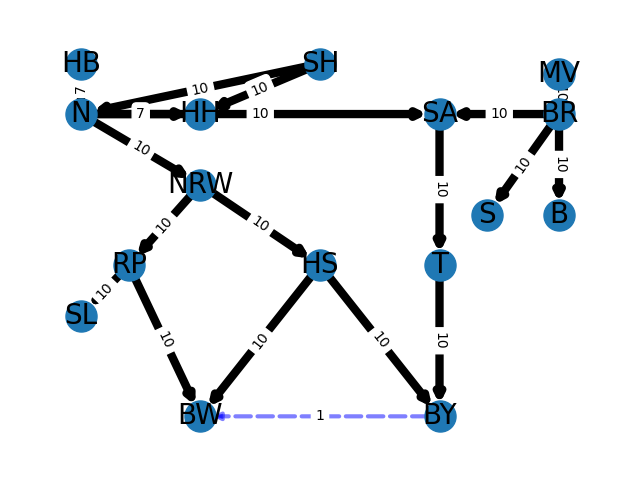
\includegraphics[width=.7\linewidth]{old_graph.png}

\end{minipage}
\end{minipage}	
		
			
		
	\end{frame}


		%---------------------------------
	\begin{frame}
		\frametitle{Graphentheoretische Herangehensweise}
		\vspace*{2mm}
		\begin{minipage}{1\linewidth}
			\begin{minipage}{.4\linewidth}
				\vspace*{-12mm}
				Max-Flow-Min-Cut:
				\begin{itemize}
					
					\item Auswertung mit Zeitreihe
						\vspace*{2mm}
					
					\item Drei Produktions- und drei Verbraucherknoten
						\vspace*{2mm}
						
					\item um Max-Flow-Min-Cut anwenden zu können:
						\vspace*{2mm}
						\begin{itemize}
							\item jeweils einem gebündelten Knoten
						\end{itemize}
					
					
						\vspace*{2mm}
					
					\item 
					
					
				\end{itemize}
		
			\end{minipage}
			\hfill
			\begin{minipage}{.6\linewidth}
				\centering
				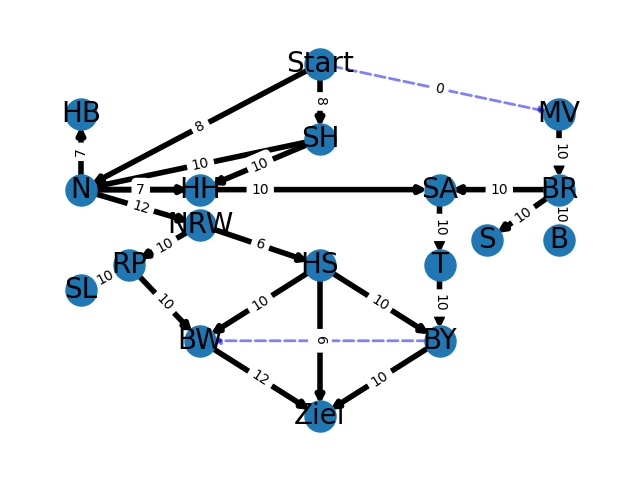
\includegraphics[width=.9\linewidth]{Figure_4.png}
				
			\end{minipage}
		\end{minipage}	
		
		
		
	\end{frame}
	
	%---------------------------------
	
	\begin{frame}
		\frametitle{Modellierung}
		\vspace*{2mm}
		\begin{minipage}{1\linewidth}
			
				\begin{itemize}
					
					\item Betrachten von zwei Länder (Deutschland, Spanien)
					
					\item Länder haben Stromproduktion und -verbrauch
					
					\item bei Überproduktion Austausch von Strom möglich 
					
					\item Bilder...
					
					
					\item
				\end{itemize}
							
		
		\end{minipage}	
		
	\end{frame}


	%---------------------------------
	\begin{frame}
		\frametitle{Modell}
		\vspace{-2mm}
		
		
		\begin{minipage}{.9\linewidth}
			\centering
			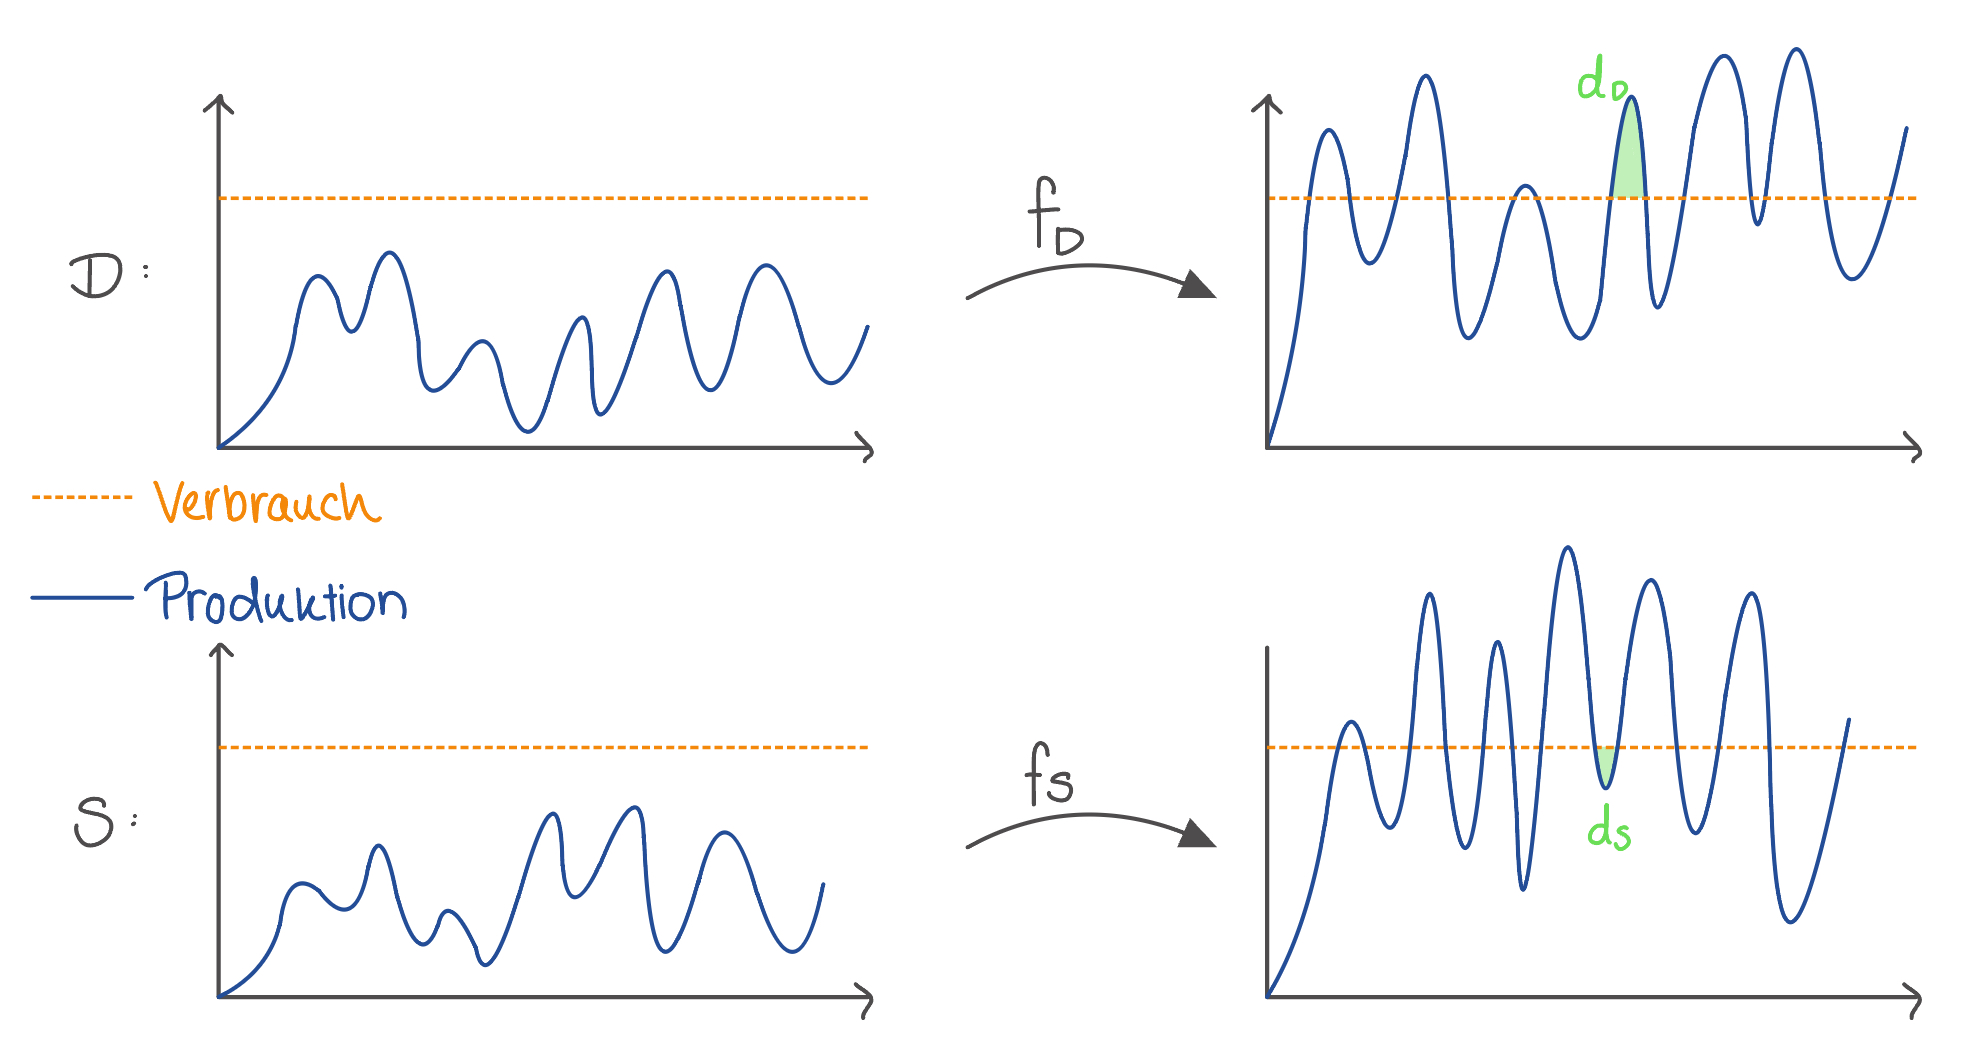
\includegraphics[width=.9\linewidth]{IMG_320.jpg}
			
		\end{minipage}
		
	\end{frame}

	%---------------------------------
	\begin{frame}
		\frametitle{Kostenfunktion}
		\vspace*{0mm}
			\begin{minipage}{1\linewidth}
			\begin{minipage}{1\linewidth}
				\begin{itemize}
					\item \begin{math}
						J(f_D, f_S, c) = (d_D + d_S) \cdot P_{Kohle} + P_{Leitung} \cdot c_{Strom} + P_{Erneuerbar}(f_D, f_S) + c_H \cdot P_H
					\end{math}
					\item 
					$	f_D$ = Skalierung der Produktion von Deutschland
					
					\item 
						$f_S$ = Skalierung der Produktion von Spanien
					\item 
					$	c$ = Kapazität
					\item 
					$	d$ = Differenz von Stromproduktion und  Stromverbrauch
					\item 
						$c_{Strom}$ (Kapazität Strom) = 
					\item \begin{math}
						c_H = -[ (\int diff) \cdot 0.6] \cdot P_{Kohle} \text{ (Kapazität Wasserstoff)}
					\end{math}
					\item \begin{math} 
						P_{Erneuerbar} = 8.4 {ct}/{kWh} \cdot \int Leistung
					\end{math}
					
				\end{itemize}
			\end{minipage}
			\hfill
			\begin{minipage}{.1\linewidth}
				\centering
				%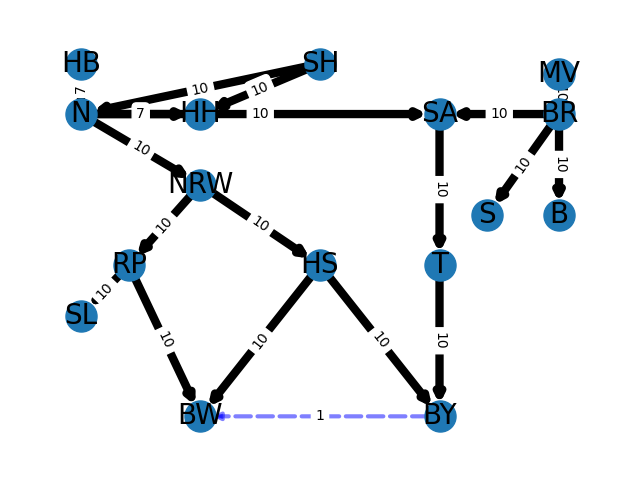
\includegraphics[width=.8\linewidth]{Example_graph_2.png}
				
			\end{minipage}
		\end{minipage}	
	
			
	\end{frame}

	%---------------------------------
		\begin{frame}
		\frametitle{Annahmen}
		\begin{itemize}
			\item
			\item Stromproduktionskosten sind fix (für Erneuerbare und Fossile Energie Produktion)
			\item Nutzung der Stromtrasse ist kostenfrei (Nur Baukosten)
			\item
			\item 
			
		\end{itemize}
	\end{frame}
	%---------------------------------
	
	\begin{frame}
		\frametitle{Ausblick}
		\begin{itemize}
			\item Graphentheoretischen Ansatz auf Modell anwenden
			\item
			\item TO do: Plotten für graphen (in und output) zwei kanten Kapazität über die Zeitreihe, wie viel läuft drüber 
			\item scipy.optimzie.minimize
			\item $x_0$ beide c´s auf null setzen, f1 = 1 = aktueller Zustand oder f1 = 3
			
		\end{itemize}
	\end{frame}
	
	


	%---------------------------------
	
	

	
	
	\begin{frame}
		\frametitle{Ausblick}
		
		\vspace*{6mm}
		\begin{itemize}
			\item erste praktische Versuche mit PyPSA bzw. Lastflussberechnungen
			\item weitere Daten suchen:
			\begin{itemize}
				\item Gasnetz (eventuell über entsog transparency platform),
				\item Bauvorhaben Wasserstoff
			\end{itemize}
			\item Kostenmodell aufstellen
			\item Unsere Stromdaten liefern verschiedene Szenarien zur Energiewende:
			
			Vielleicht reicht das für Erzeugung schon aus? 
			\item Wie genau funktioniert Import/Export?
			% \item Stahlindustrie betrachten
		\end{itemize}
			
		
	\end{frame}
	
	
	%---------------------------------
	
	
	
	
\end{document}
% eof
